\documentclass[fontsize=12pt]{article}
\linespread{1.5}
% \usepackage[margin=2.5cm]{geometry}
\usepackage[margin=2.5cm, headheight=0pt, headsep=1cm]{geometry}
\usepackage{enumerate, fancyhdr, graphicx, amsmath, float, subcaption, textcomp, hyperref, units}
\usepackage{nth}

\usepackage[binary-units=true]{siunitx}
\sisetup{load-configurations = abbreviations}

\title{Old School \tetris{} Meets Page Rank}
\author{Paul Chesnais (pmc85) \& Sam ``Sven'' Svenningsen (sjs382)}
\date{}

\def\tetris{Tetris\textsuperscript{\textregistered}}

\pagestyle{fancy}
\fancyhead{}
\lhead{pmc85 \& sjs382}
\chead{Old School \tetris{} Meets Machine Learning}
\rhead{\tetris{}}
\fancyfoot{}
\rfoot{\thepage}
\lfoot{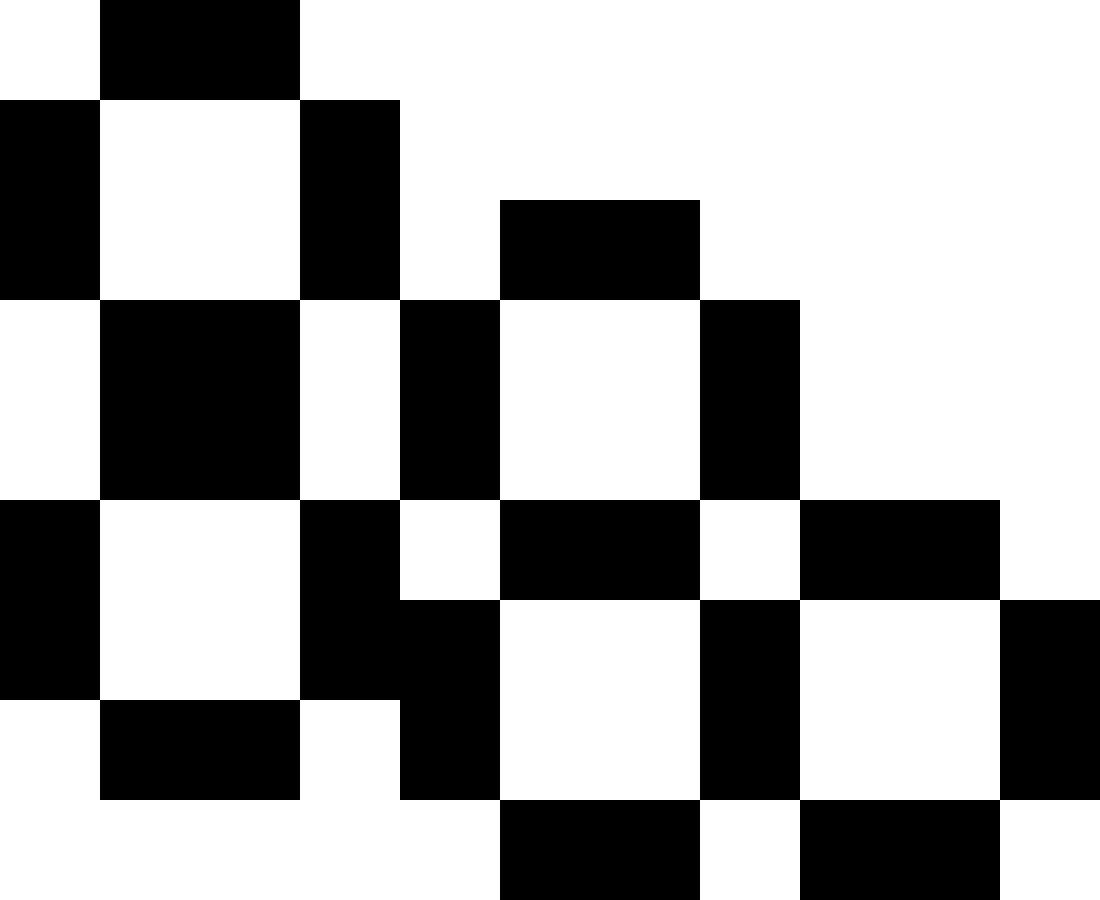
\includegraphics[height=20pt]{Logo}}
\renewcommand{\headrulewidth}{0.5pt}
\renewcommand{\footrulewidth}{0.5pt}

\usepackage{listings, color, times, textcomp, setspace}
\definecolor{Code}{rgb}{0,0,0}\definecolor{Decorators}{rgb}{0.5,0.5,0.5}\definecolor{Numbers}{rgb}{0.5,0,0}
\definecolor{MatchingBrackets}{rgb}{0.25,0.5,0.5}\definecolor{Keywords}{rgb}{0,0,0}\definecolor{self}{rgb}{0,0,0}
\definecolor{Strings}{rgb}{0,0.63,0}\definecolor{Comments}{rgb}{0,0.63,1}\definecolor{Backquotes}{rgb}{0,0,0}
\definecolor{Classname}{rgb}{0,0,0}\definecolor{FunctionName}{rgb}{0,0,0}\definecolor{Operators}{rgb}{0,0,0}
\definecolor{Background}{rgb}{0.98,0.98,0.98}

\lstdefinestyle{Scala}{
  backgroundcolor=\color{Background},basicstyle=\ttfamily\small\setstretch{1},breaklines=true,commentstyle=\color{Comments}\slshape,emph={self},emphstyle={\color{self}\slshape},frame=l,framexbottommargin=2em,framextopmargin=2em,keywordstyle={[2]\color{Decorators}\slshape},keywordstyle={\color{Keywords}\bfseries},morekeywords={abstract,case,catch,class,def,do,else,extends,false,final,finally,for,if,implicit,import,lazy,match,mixin,new,null,object,override,package,private,protected,requires,return,sealed,er,this,throw,trait,true,try,type,val,var,while,with,yield},otherkeywords={=>,<-,<\%,<:,>:,\#,@},sensitive=true,morecomment=[l]{//},morecomment=[n]{/*}{*/},morestring=[b]",morestring=[b]',morestring=[b]""",numbers=left,numbersep=1em,numberstyle=\footnotesize,showspaces=false,showstringspaces=false,showtabs=false,stringstyle=\color{Strings},tabsize=4,xleftmargin=1em,
}

\lstdefinestyle{Pseudocode}{
  backgroundcolor=\color{Background},basicstyle=\ttfamily\small\setstretch{1},breaklines=true,mathescape,
  commentstyle=\color{Comments}\slshape,emph={self},emphstyle={\color{self}\slshape},frame=l,framexbottommargin=2em,
  framextopmargin=2em,keywordstyle={[2]\color{Decorators}\slshape},keywordstyle={\color{Keywords}\bfseries},
  morekeywords={for,while,if,in,else,break,def,endfor,endif,enddef,endwhile,return,None},otherkeywords={:=, =},
  numbers=left,numbersep=1em,numberstyle=\footnotesize,showspaces=false,showstringspaces=false,showtabs=false,
  stringstyle=\color{Strings},tabsize=4,xleftmargin=1em,
}

\begin{document}
\maketitle
\thispagestyle{empty}
\section{Abstract}
\label{sec:abstract}

\par It has been shown that \tetris{}, the Russian tile-stacking puzzle video game, is NP-Complete \cite{bib:tetrishard}. This project sought to try to approximate a solution to \tetris{} that plays well according to human standards. Evidently, no solutions can be perfect (assuming $P \neq NP$), but one can still try. The current algorithm approximates a solution by ranking the contour (the shape of the top of the stack) using a method akin to Google's PageRank algorithm, then choosing the sequence of Tetrominoes (\tetris{} pieces) that lead to the highest ranking stack.

\section{Getting computers to play \tetris{}}
\label{sec:getting_computers_to_play_tetris}

\subsection{An Introduction to the Game}
\label{sub:an_introduction_to_the_game}

\begin{figure}[h!]
  \centering
  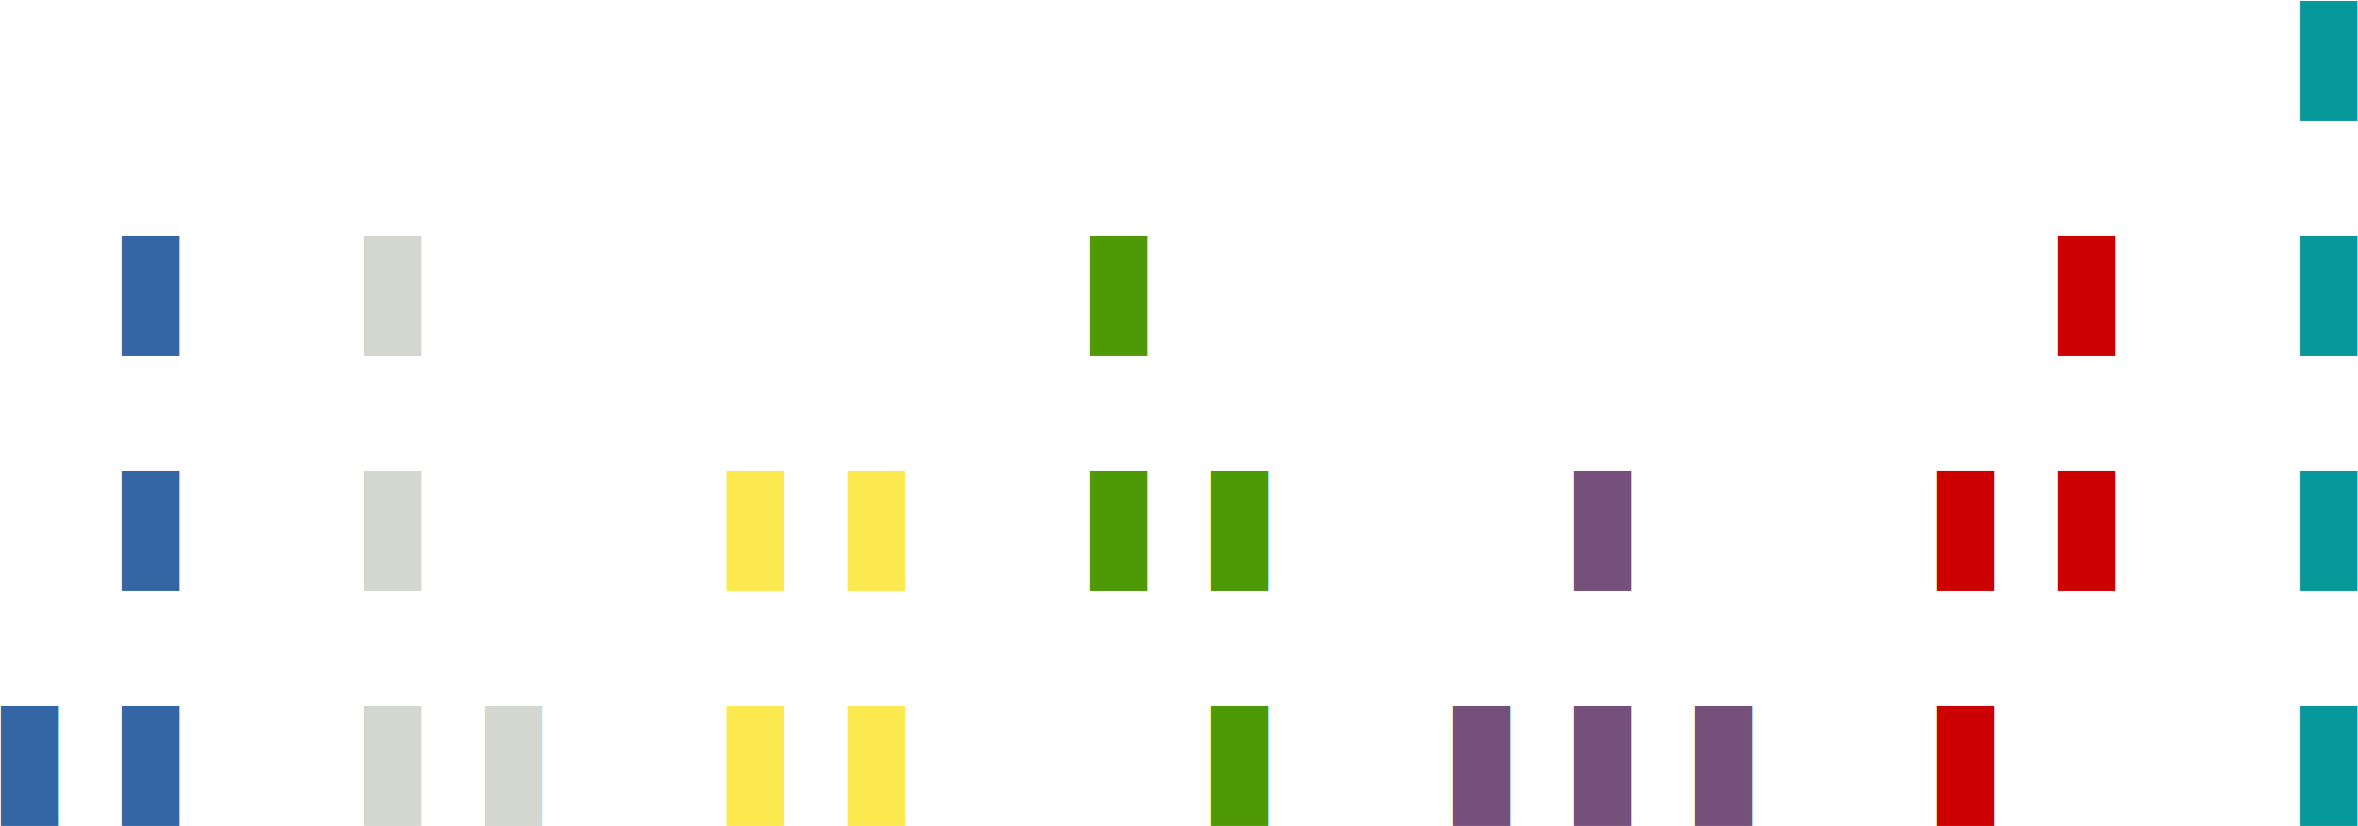
\includegraphics[width=0.4\textwidth, height=0.1\textwidth]{figures/pieces}
  \caption{The 7 tetrominoes $J$, $L$, $O$, $S$, $T$, $Z$ and $I$ }
  \label{fig:the_7_tetrominoes}
\end{figure}

\par The mechanics of \tetris{} are beautifully simple. The user begins with an game board, henceforth referred to as the ``stack'', 10 units wide and 20 units high. The user is then given a random sequence of the \tetris{} pieces, or ``tetrominoes'', shown in Figure~\ref{fig:the_7_tetrominoes}, to be placed on top of one another. Tetrominoes are each made up of 4 identical connected squares, and rotate by 90\textdegree clockwise or counterclockwise. When a tetromino is placed, it maintains its shape. In other words, it can create holes (see Figure~\ref{fig:placing_an_i_piece_to_clear_a_row}).
\par When a horizontal line is full, this line is removed. Every individual square above the cleared row then move directly downward $n$ vertical units, where $n$ is the number of row cleared. Figure~\ref{fig:placing_an_i_piece_to_clear_a_row} shows both the mechanic involved in clearing rows, and how poor placement of piece can create undesired holes. Here, the $I$ piece was placed horizontally on top of the $O$, which blocks access to the three empty spaces below.
\par As time goes on, the amount of time the user has to place the piece decreases, making it difficult to keep up with, and to keep playing, the user must clear as many rows as possible to prevent the top of the stack from reaching height 20, otherwise, it's GAME OVER. The game is scored relative to how many rows were cleared by a single placement, and how frequently rows are cleared. The best score is achieved by using the $I$ piece to clear 4 rows at once, and consecutive row clears multiply the score given (i.e. combos).

\begin{figure}[h!]
  \centering
  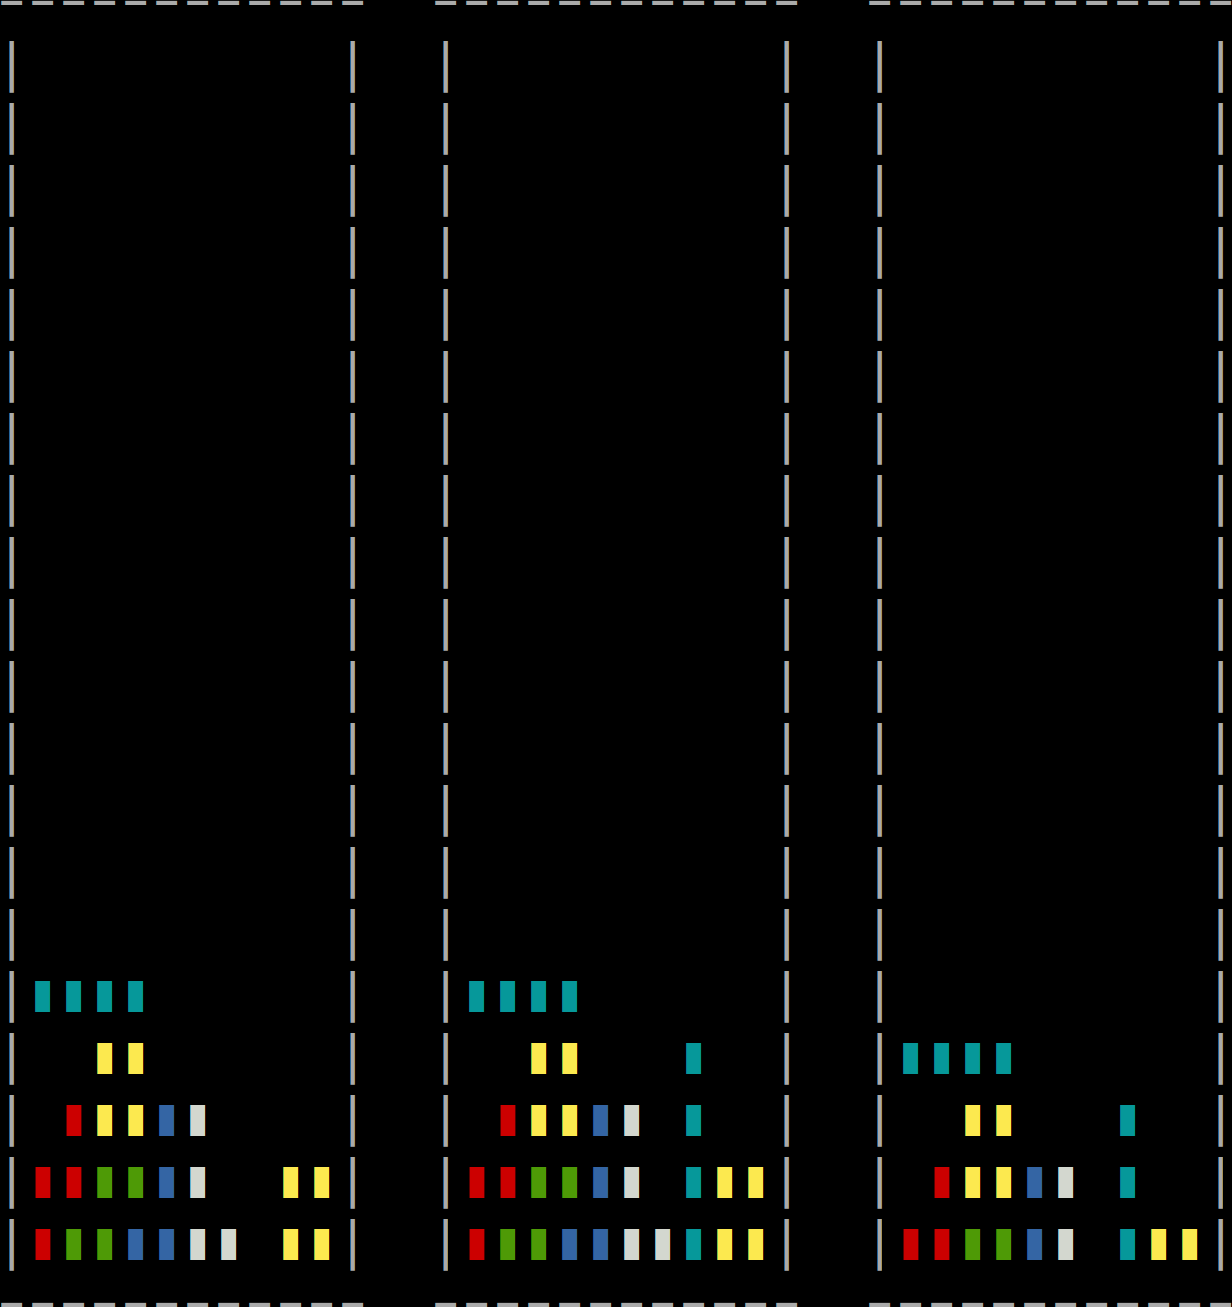
\includegraphics[width=0.6\textwidth, height=0.4\textwidth]{figures/rowclear-crop}
  \caption{Placing an $I$ piece to clear a row}
  \label{fig:placing_an_i_piece_to_clear_a_row}
\end{figure}

\subsection{Representations}
\label{sub:representations}
\subsubsection{Tetrominoes}
\label{ssub:tetrominoes}

\par A simple, yet efficient efficient way to represent an single rotation of an individual tetromino is by keeping a list of two dimensional vectors representing the location of each square from the center of mass of the tetromino. Equation~\ref{eq:t_offsets} is an example of such a list for the $T$ piece in the orientation shown in Figure~\ref{fig:the_7_tetrominoes}.
\begin{align}
  [(0,0), (-1, 0), (0, 1), (1, 0)]\label{eq:t_offsets}
\end{align}
With these lists and a given pair of coordinates $(x,y)$, finding the location of each square of a given tetromino only requires translating $(x,y)$ by each vector in the list.

\subsubsection{The Stack}
\label{ssub:the_stack}
\paragraph{Arrays}
\label{par:arrays}
One way to represent a stack is with an array. In this case, the stack was represented as a $10\times 20$ two dimensional array, where each square in the theoretical stack maps to an element in the array. One square is represented as a tuple $(s,c)$ where $s$ is a boolean representing whether or not there exists a square in the stack at that location, and $c$ is the color of that square \footnote{Again, $c$ is only kept for graphical purposes and plays no role in the actual implementation}. In this implementation, traversing the array to figure out whether or not a row is full is very straightforward.
\par Adding a tetromino to such a stack is a little more difficult. The player (human or otherwise) only has a choice between which column the center of mass of the tetromino will fall on, and at which height the piece will settle is entirely dependent on the current state of the stack. To find which height the tetromino should settle at, all we need to do is iteratively try to place the tetromino higher and higher starting at the current height of the specified column plus one. If at any time, any of the squares in the tetromino occupy a square that is already full, this height must be invalid, and we must try again one unit higher. Once all the squares fit and occupy what were empty spaces, return the new stack. This is a little slow, but is the only way to find a position where the tetromino fits.
\paragraph{Contour}
\label{par:contour}
The other way to represent a stack, according to Ryan Heise's similar attempt at playing \tetris{} \cite{bib:ryan_heise}, is by only keeping track of the shape of the stack's contour. The stack's contour is defined by the height of each individual column minus the height of the shortest column. Suppose we maintain the guarantee that the stack is always full, i.e. never has holes, and one of the outermost columns is always kept empty. In this case, two stacks of different heights can have the same contour, and all stacks with the same contour can be treated equally. Heise also introduced a method of serializing this contour to a single integer. A stack can be represented as a sequence of ``relative difference in height between one column and the next'', with the slight subtlety that an absolute difference greater than 4 will be cut to -4 and 4 accordingly. This sacrifice in complexity is argued to be mostly harmless under the guise that two such stacks will behave similarly. Given this sequence of numbers between -4 and 4, we can add 4 to each and string them together to get a base 9 integers. There is therefore a 1 to 1 mapping between contours and integers, which allows us to generate stacks without brute forcing every single possible arrangement. The flaw in this method is that it can only generate stacks that are 9 columns wide. This is by design. The reasoning behind it comes from the fact that the only way to clear rows in a completely full, 9 column wide stack without creating holes is to use an $I$ piece in the empty columns, potentially clearing 4 rows at once. A 4-row clear is called a Tetris because it is hardest to achieve and rewards the player with the most points. Therefore a player that plays only on stacks generated by this approach is likely to have the highest possible score, meaning that using this method is still acceptable.
\par We can also add tetrominoes directly to a contour, given a desired column. First, transform the contour back into a list of heights. Then, for the desired column, attempt to place the tetromino at that height plus the height of the tetromino's center of mass. For all columns of height $h$, if the tetromino adds $n$ squares to that column, check that all those squares are at height $\leq h + n$. If not, then placing the tetromino at that height must have put a hole in the stack. This violates the invariant that a contour represents a stack with no holes, and therefore that tetromino cannot be placed in this spot. This is more efficient than the addition operation described above, since there are fewer squares to check.

\subsection{Randomizer}
\label{sub:randomizer}
\par The final step in this simulation of the game is to implement the Randomizer. In \tetris{}, the Randomizer is the component that decides which tetromino the player must place on the stack next. The \tetris{} Grand Master official \cite{bib:TGMRandomizer} Randomizer is initialized as a queue containing the following 4 pieces: $Z,Z,S,S$. The queue represents the last 4 tetrominoes dealt to the user. The Randomizer then randomly picks a tetromino, each with equal chance. If the picked tetromino is in the history, the Randomizer tries again, else the new piece is pushed onto the history, the least recent piece is removed from the history, and the new piece is dealt to the user. The Randomizer attempts to generate a new piece that is not in the history six times. If all six pieces were in the history, then the Randomizer returns the most recently generated piece after pushing it onto the history, and removing the least recent piece from history.
\par The Randomizer behaves like this in order to decrease the likelihood of a given piece being dealt too many times in a row. The Randomizer also never deals an $S$ or a $Z$ as the first piece, otherwise the user is forced to have a hanging square from the very beginning.

\subsection{Relaxations}
\label{sub:relaxations}
\paragraph{Scoring}
\label{par:scoring}
The scoring scheme outlined above is unfortunately quite complex. Additionally, every implementation of \tetris{} uses a slightly different scheme. As such, given that there is no strong consensus and given the additional complexity, the decision was made to score a player by how many tetrominoes they can consecutively place without losing. This also implies that a bot can search for the best move only by looking at the expected life of the stack that it creates.
\paragraph{Timing}
\label{par:timing}
Another important aspect of \tetris{} is that there is a time limit for every move. The first problem is that it is hard to interrupt a running algorithm and get the currently computed best move from it. The second problem is that computers are quite fast, and are expected to come up with the next best move rather quickly. As such, instead of setting arbitrarily low time limits on the players, no time limits were set under the assumptions that AI players would be too fast for it to matter anyway.

% \section{Initial Attempts}
% \label{sec:initial_attempts}

% \subsection{MiniMax}
% \par We tried to maximize the pieces placement in a way that would minimize the possible damage/maximize the least expected outcome of the next few pieces the \tetris{} board provides by using the MiniMax approach.
% \subsubsection{Heuristic}
% \par This lead us into the difficulty of grading boards on quality so that we could have a function to minimize over.

% \par One thought would be to penalize boards that have holes or overhangs in them (i.e. pieces covering empty spaces), though penalize overhangs less since you can get around them sometimes.

% \par The next obvious criteria was to give a max value to any board that has a \tetris{} (4 complete rows at once) and a lesser, but still high, score to any number of complete rows.

% \par This leaves us an issue of all the boards with no obvious issues, and no obvious bonuses. We made a guess that having a more level board would be best (i.e. the distance between the lowest free spot and the highest tower you have is minimized).

% \par An alternative to this is to make up as many features as possible and try to assign weights to them based on if they lead to failed games quickly (we'd have to play the game a bunch of times).

% \par We weren't quite sure how to implement this though since we did not know how to weight each feature appropriately besides running it a million times over, which was too slow.

% \subsubsection{The Tree}

% \par We began by choosing trees that would be good regardless of what the unknown pieces would be, this meant leaving out what would probably have been good choices assuming we didn't get the one or two pieces, or combinations, that messed it up. Later, we considered weighing the loss according to its likelihood, though we were unsure how to make that work in terms of discounting the negative value of a branch.

% \par We memoized the algorithm by keeping the trees in memory and clipping relevant branches as we went on, and just recomputed the last branch from there so as to save time.

% \section{Challenges Faced}
% \label{sec:challenges_faced}

% \subsection{Size of State Space}

% \par The size of the state space leads to some issues. There are about $10-40$ places to put a piece if you know which one it is (each piece has between 1 and 4 rotations and 10 spots you can put it in), and $190$ places you can put a piece each round for an unknown piece. So to do this n-places into the unknown piece space you have about $160*190^n$ pieces, which ends up being on the order of $10^{2n + 2}$ each round, even looking 3 pieces ahead into the unknown can take $10^{8}$ possible boards to check, which does not take a trivial amount of time.

% \par This issue is made even worse for our PageRank algorithm, which has to literally check every single possible board. The size of this table ended up being larger than our RAM, so we had to write it to disk. This leads to very slow read times since it is incredibly rare that we get a cache hit (since boards don't tend to repeat anywhere near frequently enough to get hit).

% \subsection{Scala issues}

% \par Scala, a coding language that is a superset of Java, kept optimizing our for loops. It also had trouble efficiently dealing with the binary files (in terms of I/O) that we had to write our massive rankings data to.


\section{Stack Rank}
\label{sec:page_rank}

\par The current and best algorithm developed for this project uses a method that is quite close to Google's PageRank algorithm. Given an arbitrary stack, it attempts to calculate a meaningful rank given the rank of the stacks that it can reach and the stacks that reach it. For a stack $s$ to be able to ``reach'' another stack $s'$, there exists a tetromino such that can be placed on $s$ without creating any holes such that $s$ and $s'$ have the same contour.

\subsection{The Mapping Stage}
\label{sub:the_mapping_stage}

\subsubsection{In theory}
\label{ssub:in_theory}
\par The contour approximation of a stack's features can only represent $9^8$ stacks, and as such, this is how many stacks the algorithm will attempt to rank. We can think of the total set of stacks as a graph, with a directed edge connecting stack $s$ to stack $s'$ if and only if $s$ can reach $s'$. Incidentally, this graph exists independently of rank, has a very large number of nodes, and is expected to have a very high connectivity, given the fact that a single stack can potentially reach dozens of different stacks. It would therefore be ideal if this graph did not have to be recomputed. Hence the creation of the Mapping Stage.
\par The Mapping Stage computes the complete graph of stacks as a map between a stack $s$ and a tetromino $t$ to a new stack $s'$. There is a difference between this graph and the graph outlined above in that there effectively are 7 graphs, one for each tetromino, where an edge only exists between two stacks if one can reach the other using the tetromino associated with that graph. The reason for this difference is that in the Ranking Stage, the ranker needs to know what tetrominoes were used to connect the stacks. This will be addressed in Section~\ref{sub:the_ranking_stage}.

\subsubsection{Technical difficulties}
\label{ssub:technical_difficulties}
\par Suppose that on average, a given stack and a given tetromino can reach 10 different stacks. Suppose we also represent the 7 tetrominoes with a number between 0 and 6. This number can fit in one byte, and will be stored as such. Therefore each key in the map is 5 bytes long: the 32-bit integer representing the contour and the byte representing the tetromino. Additionally, each value in the map is expected to be $10 \times 4 = 40$ bytes long. The following equation is a preliminary calculation of how large the map will be:
\begin{align*}
  (9^8 \times 7) \times (5 \times 40) \simeq \SI{6.02e10}{\byte} \simeq \SI{56.127}{\giga\byte}\label{eq:map_size}
\end{align*}
Evidently, this will not fit in the memory of most machines. As such, precautions were immediately taken: the map was to be calculated piecewise. The range from 0 to $9^8$ was split into 1000 segment. For each contour in a given segment, the full mapping as defined above was computed, and stored a HashMap. Once every contour in a segment was mapped, the HashMap is forced to disk and flushed from memory. This means that, on average, the process is expected occupy less than $\SI{100}{\mega\byte}$ in memory.
\par An interesting feature of this process is that every segment can be computed independently. As such, the Mapping Stage is actually executed in parallel. Each thread/worker receives a small range of contours for which to compute the map, and said thread writes its own computed segment to disk. This greatly increased the speed of the Mapping Stage, and as such was kept as standard.
\par The final graph thankfully does not occupy \SI{56}{\giga\byte} on disk. Rather it is closer to \SI{11}{\giga\byte}. This does not change the fact that splitting it up was a good idea, but it does mean that iterating over it was a lot faster than previously projected.
% This is the reason why the map was split into 1000 segments: cache-consciousness. When one process attempts to load a large dataset from RAM into processor memory, it will evict the memory of all processes with lower or equal priority. Additionally, all the cores in a single chip share the same processor memory. As such, when multiple processes are running in parallel, they are all fighting over space. Suppose the machine has $n$ core, and $n$ threads are spawned. If the required memory for each thread is small, then the likelihood of either having their memory evicted is low. As such, is

\subsection{The Ranking Stage}
\label{sub:the_ranking_stage}
\subsubsection{In Theory}
\label{ssub:in_theory}
\par The Ranking Stage is rather elegantly simple. Given a stack $s$, and an array $a$ of all the ranks of the stacks that reach it, compute $rank(s,a)$. The spread of ranks is computed iteratively. In other words, all ranks are initially set to the same value, then for all subsequent iterations, $a$ contains the ranks computed in the previous iteration. Because the previously computed ranks are used, the current rank of a contour changes only when it is computed, so as not to give bias to ranks depending on the order in which we compute them.
\par The greatest hurdle in computing the rank of a given stack is figuring out what a good measure for the quality of a stack is. Here were the initial attempts:
\begin{description}
  \item[Naive Connectivity] For a given stack, its rank is the sum of ranks of all the stacks that it can reach. The problem with this is that some pieces fit in a lot of places on the stack. For example, the $T$ piece is likely to place many, many times in different rotations and locations. This means that this sum is quite skewed, and means almost nothing when the piece that can be attribute to most of this sum is not available to play.
  \item[Average Connectivity] For a given stack, its rank is the average rank of all the stacks that it can reach. This suffers from the same problem as Naive Connectivity. Even though the effect is lessened, if there is a truly large difference between how many times certain pieces can be placed, then this ranking still means next to nothing when the wrong piece is in play.
  \item[Majority Rules] For a given stack, its rank is defined by the following: 0 if for more than half of the tetrominoes cannot be placed on this stack without creating a hole, else the sum of the ranks that this stack can reach over the number of tetrominoes, i.e. 7. This was actually quite a good measure. The bot played far better than with the two previous ranking schema, but there was still potential for improvement, since when the agent was unlucky, it would fail miserably. In this case, all ranks are initialized to 1.
\end{description}

\par The final ranking function, Pessimistic Evaluation, was designed to account for the absolute worst case scenario. It is quite similar to Majority Rules, but sets the score to 0 when more than 0 tetrominoes cannot be placed. Essentially, if the ranking for a given stack is nonzero, it is guaranteed that the player can keep going, regardless of which piece is dealt next. In theory, after $n$ iterations of the Ranking Stage, the stacks upon which any sequence of $n$ tetrominoes can be placed without creating holes should have the highest ranks.

\subsubsection{Technical Difficulties}
\label{ssub:technical_difficulties}
\par We know that the computed ranks of only two iterations are in play at all times. As such the ranks of all but the last two iterations can be pushed to disk and flushed from memory. The array of ranks is therefore a $2\times 9^8$ two dimensional array of either single precision floats or integers, depending on the implementation. Thankfully, this is only $2 \times 9^8 \times 4 = \SI{328.5}{\mega\byte}$, which certainly fits into memory. On the other hand, the same problem as in the Mapping Stage arises when loading the stack graph into memory: it is far too big. As such, computing the ranks is equally segmented, and only \nicefrac{1}{1000}th of the graph is loaded into memory at all times. Again, because the ranks are computed iteratively, the fact that not all of it is in memory comes into play when considering the corrected of the computations.

\section{Game Tree Search}
\label{sec:game_tree_search}

\subsection{In Theory}
\label{sub:in_theory}
\par Computing the rank of every stack using the method defined above is almost equivalent to approximating the state evaluation function for \tetris{}. In other words, this means that an agent is able to play using Game Tree Search methods. Pseudocode~\ref{lst:tetris_game_tree_traversal} is the pseudo code representation of the traversal algorithm. The algorithm traverses the Game Tree using Depth First Search, but pruning stacks that have a rank of zero, or have a rank lower than what has already been explored. It also only looks at stacks that are valid, i.e. stacks that have no holes in them, and that are not lost games. Because only stacks generated using the Contour approximating were ranked, the agent will only create stacks with an empty column. The subtlety not shown in Listing~\ref{lst:tetris_game_tree_traversal} is that if the next tetromino dealt to the player is an $I$, and the highest column in the stack has a height higher than a certain factor $h$, the agent will place the $I$ in the empty column, to force to the stack to be lower than $h$.
\renewcommand{\lstlistingname}{Pseudocode}
\begin{lstlisting}[caption=\relax \tetris{} Game Tree Traversal,label={lst:tetris_game_tree_traversal}, style=Pseudocode]
$s$ := Current Stack
$d$ := Search depth
def $Search(s,\,d)$
  $bestmove$ := null
  $bestrank$ := $-\infty$
  for $t$ in $AllPositions(AllRotations($Tetrominoes$))$
    if $\neg\,GameOver(s + t) \wedge HasNoHoles(s + t) \wedge Rank(s + t) > 0 \wedge Rank(s + t) > bestRank$
      if $d > 0$
        $bestmove$, $bestrank$ = $search(s + t,\, d - 1)$
      else
        $bestmove$ = $t$
        $bestrank$ = $rank(s + t)$
      endif
    endif
  endfor
  return bestmove, bestrank
enddef
$nextmove$,_ := $Search(s,\,d)$
$Play(nextmove)$
\end{lstlisting}
\par Two things need to be mentioned about this algorithm. The first is that it only looks at the best possible rank achievable after placing $d$ tetrominoes. Some might argue that this is not accurate because the worst case scenario needs to be considered as well. Yet, at the core of the ranking algorithm sits the fact that a stack should only have a nonzero rank if and only if \textbf{all} the tetrominoes can be placed on it. This algorithm prunes those stacks, and therefore only recommends moves that lead to stacks of nonzero rank. Choosing therefore the highest ranking sequence of moves ensures the lowest likelihood of failure.
\par The second thing that needs to be mentioned regards the nature of the Tree itself. There is a large problem with this algorithm that appears at line 6, which is that the variable $t$ becomes all possible positions and rotations of each tetromino. In other words, with $1 + 2 + 2 + 2 + 4 + 4 + 4 = 19$ total possible rotations and 10 potential columns upon which the tetromino can fall, a search down to $d$ depth can potentially expand as many as $190^d$ stacks. This is less than ideal, and becomes extremely expensive very quickly.

\subsection{Tuning the Parameters}
\label{sub:tuning_the_parameters}

\subsubsection{Search Depth}
\label{ssub:search_depth}
\par The first parameter that needs to be set is the game search depth. Ideally, this would be set to an arbitrarily large number, but that's obviously impossible.
\paragraph{Memory}
\label{par:memory}
The search is done depth first search. This means that only the current path is kept in memory, and the total memory overhead is proportional to the current depth. This overhead is the size of the instruction stack. Regardless of language, this is expected to be relatively small, and therefore memory is not the limiting factor.

\paragraph{Play Time}
\label{par:play_time}
This implementation of \tetris{} does not limit the time it takes the player to decide where they will place the piece they were dealt. This does not mean that the agent should have an infinite amount of time to play. Therefore the search depth should be tuned such that the agent takes a reasonable amount of time to make its decision. In this case, given the fact that computers crunch numbers very quickly, the agent has an unfair advantage over humans, therefore an arbitrarily low bound on search time can be set. For this particular implementation, the decision was made to tune $d$ such that the agent never takes more than half of a second to make its decision.

\paragraph{Lookahead}
\label{par:lookahead}
Most modern versions of \tetris{} give players an $n$ piece lookahead. A lookahead tells the player exactly what tetrominoes will be dealt in the upcoming $n$ turns. If the agent knows what tetrominoes will be dealt next, it can also immediately prune branches that do not fit the sequence. This would bring the branching factor down to at most $4 * 10 = 40$. This is considerably smaller, and in practice drastically reduces search time.

\par With no lookahead, the agent only takes less than half a second to make its decision when the search depth is 5. As such, this is what this parameter was set to. On the other hand, the lookahead length is expected only to make the agent's decision easier. This was indeed observed as there was a correlation between how the long the lookahead was and how long the agent was able to play without losing the game. See Figure~\ref{fig:n_lookahead_vs_play_time} for a table that demonstrates this correlation.

\subsubsection{Maximum Allowed Stack Height}
\label{ssub:maximum_allowed_stack_height}
\par The other parameter that needed to be set was the maximum allowed stack height. Letting the stack run higher means letting the agent use the $I$ tetromino longer. Since we do not know if the $I$ piece is essential to the agent's strategy (it may play a large role in constructing stacks upon which many tetrominoes can be placed), we also cannot force it to shorten the stack too early by making it place the $I$ pieces in the empty column. Therefore this parameter needs to be tuned as well. This parameter was set using empirical evidence. The agent was given a 5 piece lookahead, i.e. the best possible lookahead given that its search depth is 5, and played the game multiple times over, with instruction to limit the stack height at particular values. Figure~\ref{fig:maximum_stack_height_vs_time_alive} shows the relationship between the stack height and how many consecutive pieces the agent was able to place without losing.

\begin{figure}[H]
  \centering
  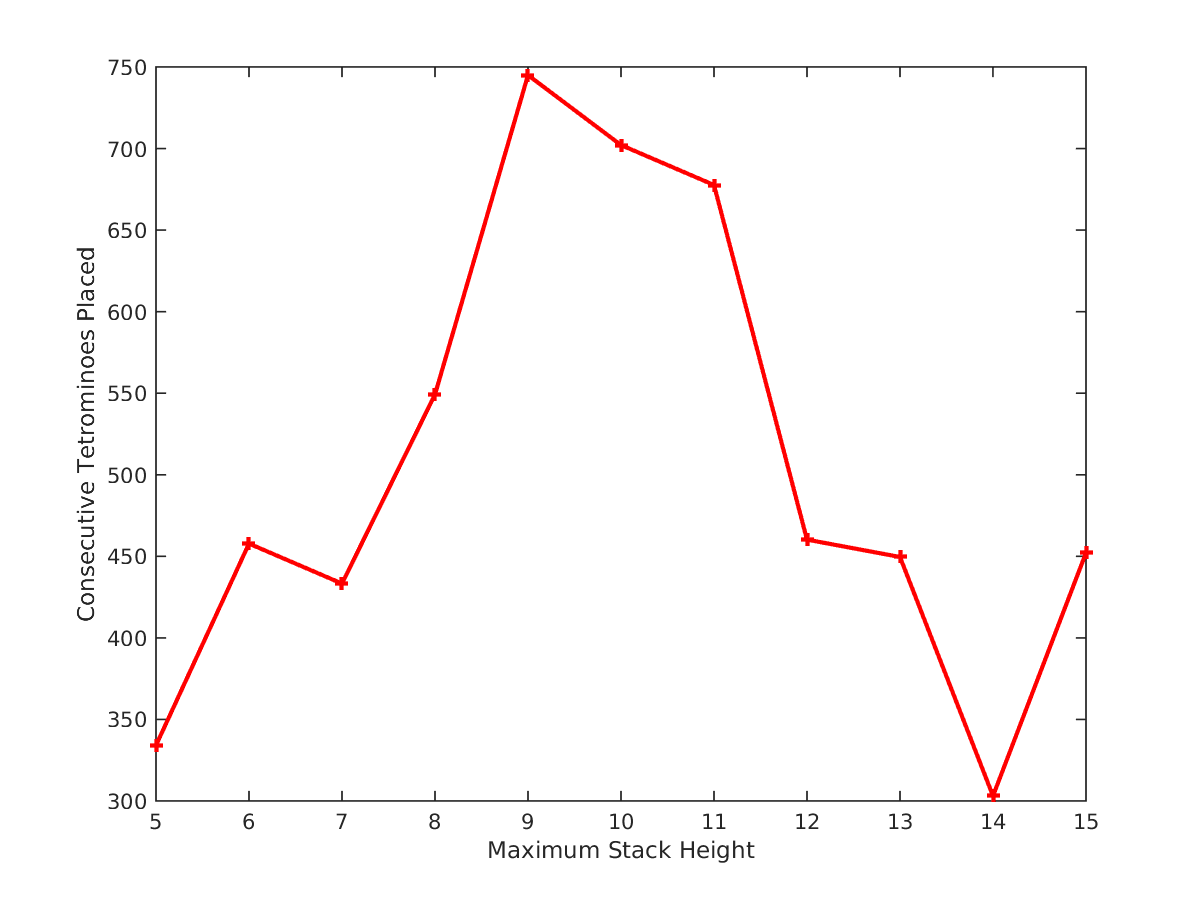
\includegraphics[width=0.5\textwidth]{figures/height_v_time_d4}
  \caption{Maximum Stack Height versus Time Alive}
  \label{fig:maximum_stack_height_vs_time_alive}
\end{figure}

\section{Conclusion}
\label{sec:conclusion}



\newpage


\begin{thebibliography}{9}
\bibitem{bib:tetrishard}
Erik D. Demaine, Susan Hohenberger, David Liben-Nowell
\textit{
Tetris is Hard, Even to Approximate}.
\\\href{https://arxiv.org/abs/cs/0210020}{arXiv:cs/0210020}
\bibitem{bib:ryan_heise}
  \url{http://www.ryanheise.com/tetris/tetris_artificial_intelligence.html}
\bibitem{bib:world_record}
  \url{http://www.nintendolife.com/news/2012/02/new_york_gamer_breaks_tetris_record}
\bibitem{bib:TGMRandomizer}
  \url{http://tetris.wikia.com/wiki/TGM_randomizer}
\end{thebibliography}
\end{document}
